\section{Tema 1: Bølger og Bølgefunksjoner}
\label{tema1}
Dette er første samtale tema, det omfavner \textbf{prosjekt 1}. Dette inkluderer video forelesningene fra BB, se \textbf{tema 1}, \textbf{tema 2} og \textbf{tema 3}.

\autoref{tab:samtalePunkt_tema1} viser en tabell over samtale temaene, den inneholder en fargekode som representerer hvor godt jeg behersker samtaletemaet. \color{red}{Dårlig}, \color{blue}{ok, men ikke stabil} \color{black}{og} \color{teal}{Jeg er klar for eksamen}.

\color{black}
Målet er at alle temaene skal være grønne og dermed klar til eksamen.

\begin{table}[!htb]
    \centering
    \caption{Samtale punkter}
    \begin{tabular}{|c|c|c|r|}
      \hline
      1 & Ulike former for bølger &  \autoref{sec:tema1_1} & \cellcolor{blue}\quad\quad \\
      \hline 
      2 & Bølgeligningen i en dimenssjon & \autoref{sec:tema1_2} & \cellcolor{blue} \\
      \hline
      3 & Harmoniske bølger & \autoref{sec:tema1_3} & \cellcolor{blue} \\
      \hline
      4 & Stående bølger & \autoref{sec:tema1_4} & \cellcolor{green} \\
      \hline 
      5 & Bølgepakker & \autoref{sec:tema1_5} & \cellcolor{blue} \\
      \hline
      6 & Schrödingerligningen & \autoref{sec:tema1_6} & \cellcolor{green} \\ 
      \hline
      7 & Bølgefunksjonen & \autoref{sec:tema1_7} & \cellcolor{blue} \\
      \hline
      8 & Heisenbergs usikkerhets prinsipp & \autoref{sec:tema1_8} & \cellcolor{green} \\
      \hline
      9 & Dobbelspalte eksperimentet & \autoref{sec:tema1_9} & \cellcolor{green} \\
      \hline
    \end{tabular}
    \label{tab:samtalePunkt_tema1}
\end{table}

\subsection{Ulike former for bølger}
\label{sec:tema1_1}
En bølger er forstyrrelse som beveger seg eller \textbf{propagerer} vekk fra kilden, kilden i denne sammenhengen er systemet som produserer bølgen \cite{waves}. Bølger deles inn i to hovedkategorier; Mekaniske bølger og Elektromagnetiske bølger. Mekaniske bølger trenger et medium for å propagere, mens elektromagnetiske bølger ikke trenger et medium.


\begin{definition}
    \label{def:wave}
    Bølger transporterer energi uten å transportere masse.
\end{definition}

Eksempler på mekaniske bølger er bølger på en \textbf{streng}, \textbf{vannbølge} eller \textbf{lydbølge}. Fellesnevneren her er mediumet. For bølgen som beveger seg gjennom strengen er mediumet strengen selv, lydbølgen har luften som medium og vannbølgen har vannet.

Eksempler på elektromagnetiske bølger er \textbf{synlig lys}, \textbf{radiobølger} og \textbf{røntgenstråling}. Som nevnt over er ikke det ikke behov for et medium når en elektromagnetisk bølge beveger seg. Dette er fordi elektromagnetiske bølger består av osillerende elektriske og magnetiske felt, dette gjør at de kan propagere gjennom vakuum. \autoref{fig:bølgeTre} viser eksempler på bølger som inngår i hver hovedkategori.

\begin{figure}[!htb]
    \centering
    \includegraphics[scale=0.15]{Bilder/SamtaleTema1/BølgeFordeing.jpeg}
    \caption{Eksempel på bølger som som inngår i mekansike og elektromagnetiske bølger. Elektromagnetiske bølger har ingen longitudinale bølger}
    \label{fig:bølgeTre}
\end{figure}


\begin{definition}
\label{def:Transversale}
    \textbf{Transversale} bølger propagerer slik bølgemønsteret er vinkelrett på retningen til bølgen.
\end{definition}

\begin{definition}
\label{def:longitudinale}
    \textbf{Longitudiale} bølger beveger seg som bølger med sammentrykning. Longitudinale bølger beveger seg parallelt med retningen på propageringen.
\end{definition}

\begin{definition}
\label{def:ståendeBølge}
    \textbf{Stående bølger} er bølger der bølgemønsteret ser ut til å 'stå stille'.
\end{definition}

\autoref{fig:transversalBølge} viser hvordan en transversal bølge vil se ut, den blir i dette tilfellet produsert ved å bevege strengen vertikalt. Ved bruk av høyrehånden kan man se at dette skjer vinkelrett på bevegelsesretningen, la pekefinger peke i bevegelsesretning, og tommel peker opp i retningen av bølgemønsteret. \autoref{fig:longitudinalBølge} viser en longitudinal bølge, denne produseres ved å lage en horisontal bevegelse, den longitudinale bølgen beveger seg parallelt med bevegelsesretningen til bølgen. 

\begin{figure}[!htb]
    \centering
    \includegraphics[scale=0.7]{Bilder/SamtaleTema1/TransversaleBølge.png}
    \caption{Transversal bølge. \cite{waves}}
    \label{fig:transversalBølge}
\end{figure}


\begin{figure}[!htb]
    \centering
    \includegraphics[scale=0.7]{Bilder/SamtaleTema1/LongitudinalBølge.png}
    \caption{Longitudinal bølge. \cite{waves}}
    \label{fig:longitudinalBølge}
\end{figure}

Definisjon \ref{def:ståendeBølge} beskriver den stående bølgen, en stående bølge har det vi kaller noder, og antinoder. Noder er punktene som står stille i rommet, dvs de ikke har noe utslag. Antinoder er som navnet tilsier det motsatte av noder, dette er punktene som beveger seg mest, med andre ord utsvinget er størst. \autoref{fig:ståendeBølgeFig} viser tre stående bølger. Viktig ting å poengtere for stående bølger er at en stående bølge kun kan oppstå dersom begge sider er avgrenset, randbetingelsene for bevegesle i et eller begge ytterpunktene er null.

\begin{figure}[!htb]
    \centering
    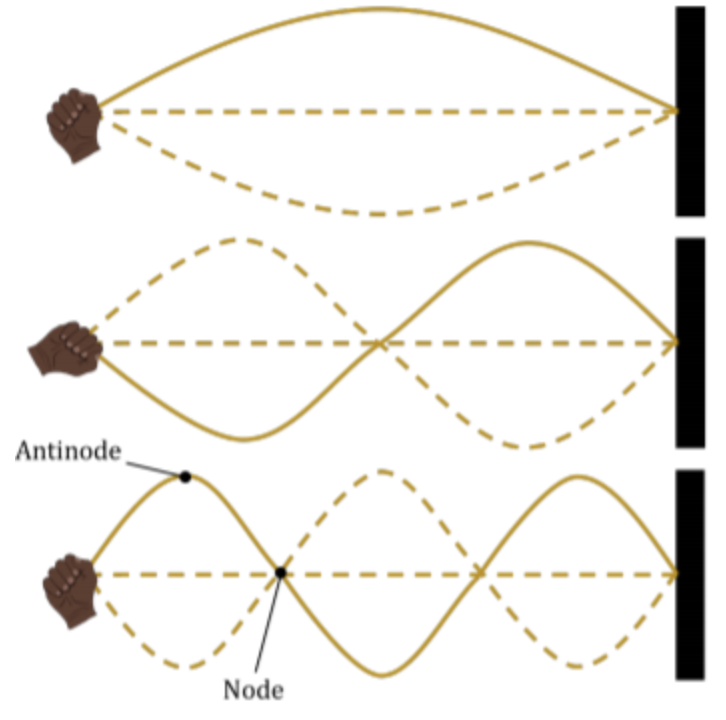
\includegraphics[scale=0.5]{Bilder/SamtaleTema1/sttåendeBølger.png}
    \caption{De tre første harmonene av stående bølger.}
    \label{fig:ståendeBølgeFig}
\end{figure}

\subsection{Bølgeligningen i en dimensjon}
\label{sec:tema1_2}
For å kunne beskrive bølgene som ble snakket om i \autoref{sec:tema1_1}, trenger man en matematisk modell som kan brukes til å beskrive og forstå bølgefenomener. Dette inkluderer lys, bølger på en streng osv. For å utlede bølgefunksjonen starter vi med å se på en enkel bølge. \autoref{fig:enkelBølge} viser en enkel sinus bølge, det røde rektangelet viser at vi ser nøye på en liten del av bølgen, dette er grunnlaget til skissen i figur \ref{fig:utledning_BL1D}, fremover blir bølgen refferert til som en streng.

\begin{figure}[!htb]
\begin{tikzpicture}
    \node[anchor=south west,inner sep=0] (image) at (0,0) {\includegraphics[width=0.9\textwidth]{Bilder/SamtaleTema1/bølgeDesmso.png}};
    \begin{scope}[x={(image.south east)},y={(image.north west)}]
        \draw[red,ultra thick,rounded corners] (0.6,0.55) rectangle (0.65,0.6);
    \end{scope}
\end{tikzpicture}
\caption{Enkel sinus bølge}
\label{fig:enkelBølge}
\end{figure}


\begin{figure}[!htb]
    \centering
    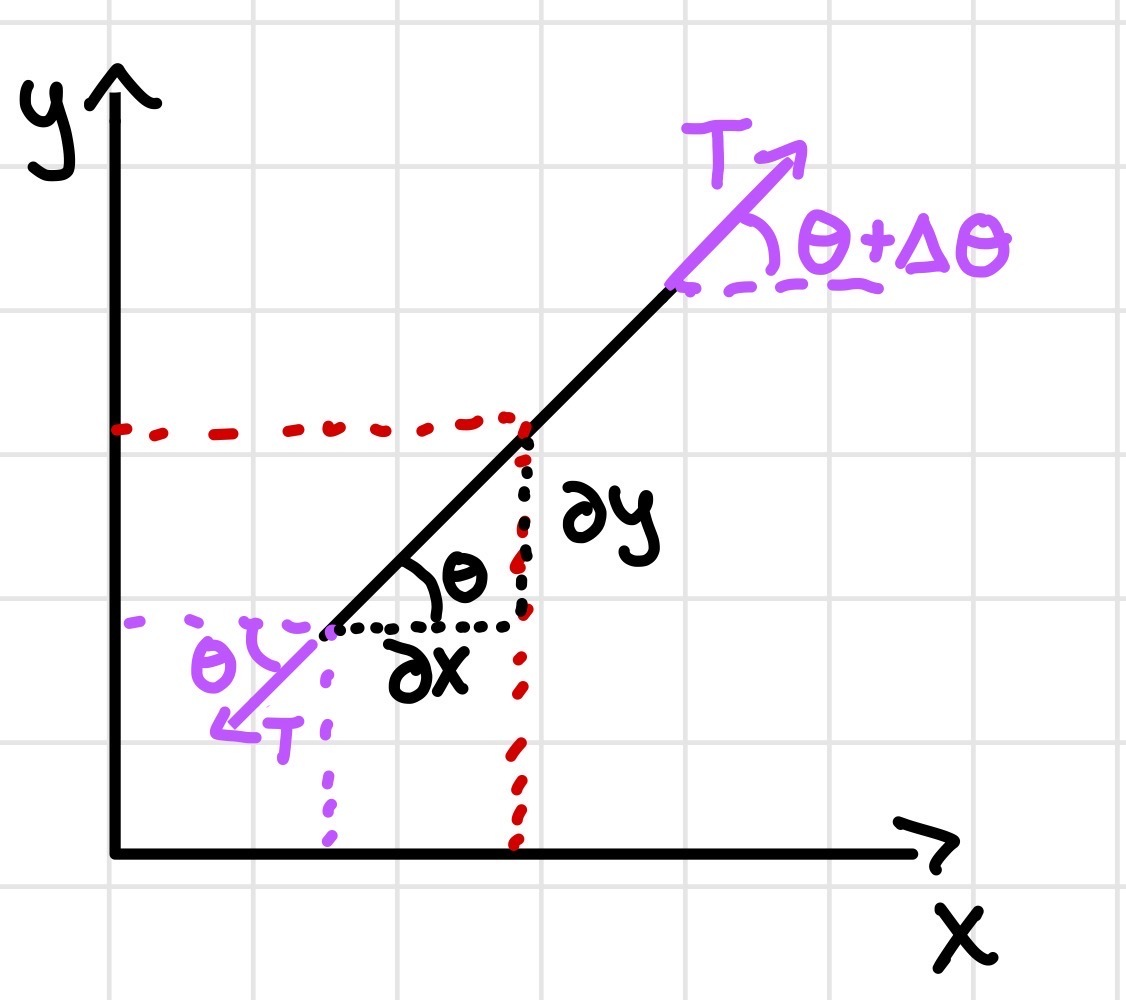
\includegraphics[scale=0.2]{Bilder/SamtaleTema1/utledning.jpeg}
    \caption{Utklipp av bølgen fra figur \ref{fig:enkelBølge}}
    \label{fig:utledning_BL1D}
\end{figure}

I tifellet fra figur \ref{fig:utledning_BL1D} er \color{red}T \color{black} snorkraften. Strengen har en masse, vi definerer denne som $\mu$ og har enhet $\bigg[\frac{kg}{m}\bigg]$. Vi kan si at delen av strengen vi ser på har lengde $\Delta x$, dermed er massen $m$.

\begin{equation}
    m = \mu \Delta x
\end{equation}

Vi ser på kreftene i y-retning, og tar i bruk småvinkel approksimasjon siden vi ser på et lite intervall.

\begin{equation}
    \begin{split}
        F_y &= -Tsin(\theta) + Tsin(\theta + \Delta)\\
        &\approx -T\theta + T\theta + T\Delta\theta
    \end{split}
\end{equation}

Siden $F=ma$, får vi at høyre side blir lik:

\begin{equation}
\label{eq:tema1_lhs}
    F_y = \mu \Delta x \frac{\partial^2y}{\partial t^2}
\end{equation}

og ved bruk at et triks\footnote{$tan(\theta)=\frac{\partial y}{\partial x} \implies$ deriver mhp. x og bruk småvinkelapproximasjon $\implies \Delta \theta =\Delta x \frac{\partial^2 y}{\partial x^2}$} kan vi skrive høyresiden

\begin{equation}
\label{eq:tema1_rhs}
    F_y = T \Delta x \frac{\partial^2y}{\partial x^2}
\end{equation}

Setter vi sammen ligning \ref{eq:tema1_lhs} og ligning \ref{eq:tema1_rhs} får vi

\begin{equation}
\label{eq:variantBL1D}
    \frac{\mu}{T} \frac{\partial^2 y}{\partial t^2} = \frac{\partial^2 y}{\partial x^2}
\end{equation}

\autoref{eq:variantBL1D} er en variant av bølgeligningen, generelt er $f(x \pm ct) $ en løsning på bølgeligningen, der $c = \sqrt{\frac{T}{\mu}}$, $c$ har dermed benevning $\big[\frac{m}{s}\big]$. Dette representerer farten til bølgen. Derfor er det vanligere å bruke $v$ istedet for $c$, da det er mer generelt og c brukes ofte for lysfarten (farten til elektromagnetiske bølger i vakum). Med det får man den mer generelle formen på den endimensjonale bølgeligningen sett i ligning \ref{eq:BL1D}.

\begin{empheq}[box=\tcbhighmath]{align}
    \label{eq:BL1D}
    \frac{1}{v^2} \frac{\partial^2 y}{\partial t^2} = \frac{\partial^2 y}{\partial x^2}
\end{empheq}

Dersom utledningen har litt hull og ikke gir full forståelse, se denne videoen \MYhref{https://www.youtube.com/watch?v=ub7lok-JQJE}{Bølgeligningen i 1D for nybegynnere}.


\newpage
\subsection{Harmoniske bølger}
\label{sec:tema1_3}
Den enkleste bølgen er den harmoniske bølgen (eller sinusbølge)\footnote{I tilfellet for osillatorer og bølger er disse synonymer.} Harmoniske bølger får man på formen vist i ligning \ref{eq:harmonicEQ}.

\begin{empheq}[box=\tcbhighmath]{align}
    \label{eq:harmonicEQ}
    u(x,t) = A\cdot cos(kx - \omega t + \phi)
\end{empheq}

En bølge har en periode, en periode $T$ er definert som tiden det tar fra et punkt på bølgen 'gjentar' seg. Bølgelengden $\lambda$ til en bølge er definert som avstanden i meter mellom to ekvivalente punkt eller med andre ord avstanden på en periode $T$. I tilfellet for ligning \ref{eq:harmonicEQ} er $k$ bølgetallet, og har et invers proporsjonalt forhold med bølgelengden, $k=\frac{2\pi}{\lambda} = [\frac{1}{m}]$. $f$ er frekvensen til bølgen, $f=\frac{1}{T}=[\frac{1}{s}]$ og kan tenkes på som hvor mange ganger i sekundet bølgen kommer med samme informasjon. $\omega$ er vinkelfrekvensen, denne er proporsjonal med frekvensen til bølgen, $\omega = 2\pi f = [\frac{rad}{s}]$. $\phi$ er faseforskyvningen til bølgen, dvs. hvor mye bølgen har blitt ''dyttet'' fra sin originale startverdi. Sist men ikke minst har vi amplituden til bølgen, siden $cos(...)$ kun innehar verdier som oppfyller ulikheten $| cos(...)|<1$, må vi ha noe som påvirker amplituden, dette er $A$, $A$ er en konstant\footnote{Dersom man vil legge til f.eks en dempningsfaktor kan man gange den harmoniske bølgen med en eksponentsialfunksjon $e^{-t\alpha}$ der alpha er en dempningskonstant.}.

Formalisme mtp. hvordan man skriver bølgefunksjonen er valgfritt, dersom man velger å bruke sinus er det snakk om et faseskift på $\frac{\pi}{2}$. Dersom $\phi$ er negativ ser det ut som bølgen forskyves mot høyre (dersom de andre verdiene i bølgen er negative). så vi kan dermed si at $sin(x) = cos(x -\frac{\pi}{2})$.

Når man skal regne med sinuser og cosinuser kan det bli vanskelig og man må ha god kontroll på trigonometriske identiteter for å kunne forenkle uttrykk. Det finnes heldigvis en annen måtte å regne på bølger, dette er ved bruk av \textbf{Eulers formel} som vi ser i ligning \ref{eq:euluers}.

\begin{equation}
    \label{eq:euluers}
    e^{i\alpha} = cos(\alpha) + isin(\alpha)
\end{equation}

Ved bruk av ligning \ref{eq:harmonicEQ} og ligning \ref{eq:euluers} kan vi skrive om uttrykket vi har for harmoniske bølger og vi får ligning \ref{eq:omskrivningHarmonic}

\begin{empheq}[box=\tcbhighmath]{align}
    \label{eq:omskrivningHarmonic}
    Acos(kx-\omega t + \phi) = \Re\bigg(Ae^{i(kx-\omega t + \phi}\bigg)
\end{empheq}

Siden vi som oftest jobber med klassiske bølger dropper vi $\Re$, dette er fordi den klassiske harmoniske bølgen ikke inneholder noen imaginære bidrag.
\newpage
\subsubsection{Gruppe- og Fasehastighet}
\textbf{Gruppehastighet} er hastigheten til en bølgepakke som beveger seg gjennom et medium. 
\begin{equation}
    \label{eq:gruppv}
    v_g = \frac{\partial \omega}{\partial k}
\end{equation}

\textbf{Fasehastigheten} til en bølge er ''rate at which the wave propogates in any medium.'', 

\begin{equation}
    \label{eq:fasev}
    v_p = \frac{\lambda}{T} = \frac{\omega}{k}
\end{equation}
Bruk gjerne animasjonene fra \MYhref{https://en.wikipedia.org/wiki/Group_velocity}{Wikipedia} for visualisering av konseptet, for en harmonisk bølge er disse to like.
\subsubsection{Viser regning}
Dette er tilleggsmateriell og ikke helt nødvendig for pensumet i faget (anno. 2024). 

En viser er en representasjon av en sinusformet bølge med amplitude, A, fasekonstant, $\phi$, og vinkelfrekvens, $\omega$, er uavhengig av tid (tidinvariant). Tidsinvariansen gir oss følgende definisjon:

\begin{equation}
    \label{eq:viser}
    Asin(\omega t +\phi) = \Re\bigg(Ae^{i\phi}e^{i\omega t}\bigg)
\end{equation}

Vi kan her si at $\textbf{v} = Ae^{i\phi}$ er viseren, denne ''spinner'' rundt i det komplekse plan som en funksjon av tid. selvom viseren ikke har en tidsvariabel er dette en metafor for å hjelpe på forståelsen av viseren. $\textbf{V}$ er et imaginært tall som inneholder informasjon om amplituden og fase vinkelen til den gitte sinus funksjonen \cite{EC10th}. \autoref{fig:viserPlot} er en illustrasjon som skal vise hva som har blitt skrevet i dette avsnittet, dette er vanskelig så se gjerne på fler ressurser på internett for bedre forklaringer.

\begin{figure}[!htb]
    \centering
    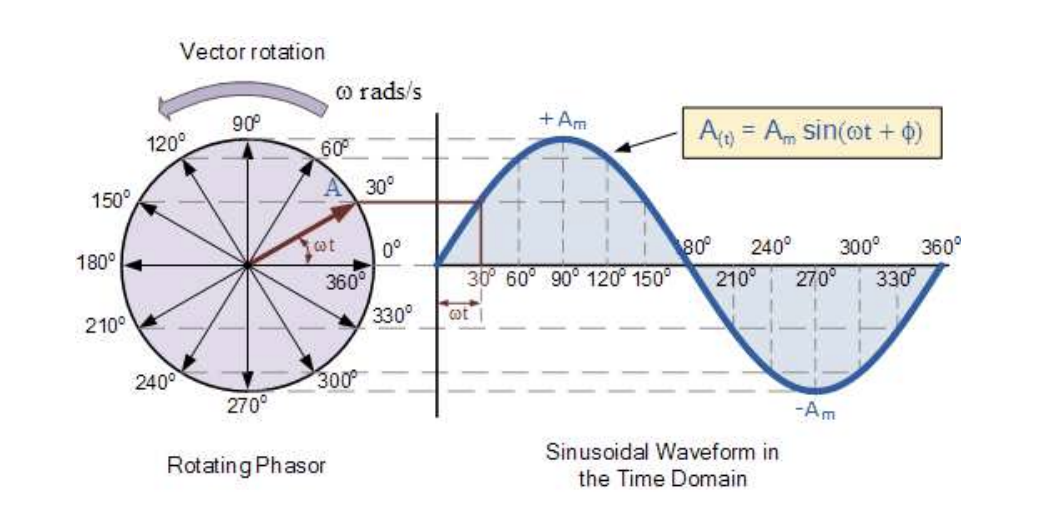
\includegraphics[scale=0.7]{Bilder/SamtaleTema1/viser.png}
    \caption{Henter fra Electronics tutorials \cite{electronics}.}
    \label{fig:viserPlot}
\end{figure}


\newpage
\subsection{Stående bølger}
\label{sec:tema1_4}
Vi skal legge litt mer informasjon til i definisjonen vår av stående bølger fra \autoref{sec:tema1_1}. Vi kan definere en stående bølge som vi har gjort i definisjon \autoref{def:ståendeBølge}, men vi kan også definere det som definisjon \autoref{def:ståendeBølge2}.

\begin{definition}
    \label{def:ståendeBølge2}
    Kombinasjon av to bølger som beveger seg i \textbf{motsatte} retninger. Begge har samme amplitude og frekvens
\end{definition}

En konsekvens av informasjoen fra definisjon \ref{def:ståendeBølge2} er at bølger som ''kolliderer'' med hverandre vil gi opphav til fenomenet interferens, dette gjør at superposisjnen av bølgene vil enten øke den totale bølgeamplituden eller minke den, hhv. konstruktiv og destruktiv interferens. 

Vi tar et eksempel, la oss si vi har to bølger, de er definert i ligning \ref{eq:u1} og ligning \ref{eq:u2}.

\begin{equation}
    \label{eq:u1}
    u_1(x,t) = Acos(kx+\omega t)
\end{equation}
\begin{equation}
    \label{eq:u2}
    u_2(x,t) = Acos(kx-\omega t)
\end{equation}

Vi ser at ligning \ref{eq:u1} og \ref{eq:u2} har to bølger som beveger seg likt i rommet, men ulikt i tid. Dersom vi tar i bruk superposisjonsprinsippet kan vi si at summen av de energien fra de to bølgene er det den totale påvirkningen på omgivelsene.

\begin{equation}
    \label{eq:superpos}
    \begin{split}
        u(x,t) &= u_1(x,t) + u_2(x,t)\\
        &= Acos(kx+\omega t) + Acos(kx-\omega t)\\
        &= 2A cos(kx) cos(\omega t)
    \end{split}
\end{equation}

Resulatet fra \autoref{eq:superpos} produserer en bølge vi kaller en stående bølge, denne består av en bølge $cos(kx)$, denne varierer i rom, og vi har $cos(\omega t)$ som vil variere i tid.

\begin{gather*}
    \begin{split}
    &\text{Avstand mellom to noder: $\frac{\lambda}{2}$}\\
    &\text{Avstand mellom node og antinode: $\frac{\lambda}{4}$}
    \end{split}
\end{gather*}

For en stående bølge er det ingen energitransport, et annet vanlig navn for denne type bølge er ''Stasjonær bølge''.
\newpage

\subsection{Bølgepakker}
\label{sec:tema1_5}
En bølgepakke er en sammensatt bølge, pakken består da av en superposisjons av bølger, dvs:

\begin{equation}
    U(x,t) = \Sigma_{k=1}^N u_k(x,t)
\end{equation}

Bølgepakken vil bevege seg med gruppehastigheten til bølgen $v_g$. Dersom to forskjellige bølger er løsninger på bølgeligningen (\ref{eq:BL1D}), vil summen av de to også løse ligning \ref{eq:BL1D}. Dersom systemene ikke er lineære stemmer ikke dette, en enkel forklaring på dette er at addering er en lineær operasjon.

\subsection{Schrödingerligningen}
\label{sec:tema1_6}
De-Broglie postulerte i sin PhD oppgave fra 1924 at akkurat som lys hadde både partikkel og bølge egenskaper. Ville elektroner også ha bølge egenskaper. Resulatet mot slutten av PhD oppgaven er dette kjente uttrykket: 

\begin{equation}
    \label{eq:debroglie1}
    \lambda = \frac{h}{p}
\end{equation}

\autoref{eq:debroglie1} inneholder informasjon om partikkelens bølgelengde $\lambda$, og bevegelseslmengde $p$. Plancks konstant $h$ innehar omtrent verdien $6.63\cdot10^{-34}\,\si{\joule\per\second}$. Uttrykket kan skrives om til ligning \ref{eq:debroglie2} ved bruk av $k=\frac{2\pi}{\lambda}$ og $\hbar = \frac{h}{2\pi}$.

\begin{equation}
    \label{eq:debroglie2}
    p = \hbar k
\end{equation}

Ved å si at partikkeler har bølge egenskaper kan vi skrive om engergien ved hjelp av frekvensen, akkurat som for lys.

\begin{equation}
    \label{eq:energy}
    E = hf = \frac{h\omega}{2\pi}=\hbar\omega
\end{equation}

Vi må beskrive bølgene våre også, vi tar i bruk det vi så på i \autoref{sec:tema1_3} om harmoniske bølger, og vi skriver derfor en 3D bølge slik som i ligning \ref{eq:bølgefunc3D}

\begin{equation}
    \label{eq:bølgefunc3D}
    \Psi(\textbf{r},t) = e^{i(\textbf{k}\textbf{r}-\omega t)}
\end{equation}

I en dimensjon skriver vi det som i ligning \ref{eq:bølgefunc1D}
\begin{empheq}[box=\tcbhighmath]{align}
    \label{eq:bølgefunc1D}
    \Psi(x,t) = e^{i(kx -\omega t)}
\end{empheq}

I 1925 postulerte shrödinger en ligning utifra hva De-Broglie hadde funnet om ''materie bølgen''. Han kom fram til ligning \ref{eq:shrodinger}

\begin{empheq}[box=\tcbhighmath]{align}
    \label{eq:shrodinger}
    i\hbar \frac{\partial \Psi}{\partial t} = \hat{H}\Psi
\end{empheq}

Her er $\Psi$ bølgefunksjonen som ble beskrevet i ligning \ref{eq:bølgefunc1D}. Ved bruk av shrodinger ligningen kan man finne en rekke verdier som forklarer en bølge $\Psi$ er en bølgefunksjon som løser shrödiner ligningen. Vi kan bruke det som et eksempel til å finne bevegelsesmengden $p$, men for å finne $p$ må vi anvende en operator. $p=\hbar k$, så hvis vi deriverer $\Psi$ mhp $x$ er vi et steg nærmere.

\begin{equation}
    \frac{\partial}{\partial x}\Psi(x,t) = ik \cdot e^{i(kx-\omega t)}
\end{equation}

Vi er et steg nærmere ja, men vi har en $i$ her og vi mangle $\hbar$, så la oss modifisere operatoren så den ganger med $\hbar$ og deler på $i$.

\begin{equation}
    \frac{\hbar}{i}\frac{\partial}{\partial x}\Psi(x,t) = \hbar k \Psi(x,t) = p\Psi(x,t)
\end{equation}

Vi får ved bruk av operatoren $\hat{P}$ ut $p$, her er $p$ en reell tallverdi. Når en operator anvendt på en bølgefunksjon 'stemmer' sier vi at $\Psi(x,t)$ er en egentilstand av $\hat{P}$ med egenverdi $p$.

\begin{empheq}[box=\tcbhighmath]{align}
    \label{eq:bevegelsesmengdeOperator}
    \hat{P} = \frac{\hbar}{i} \frac{\partial}{\partial x}
\end{empheq}

Vi kan gjøre det samme for energien, vi vet at den kan bli skrevet på formen som ligning \ref{eq:energy}. Vi får dermed at 

\begin{equation}
    \begin{split}
    i\hbar \frac{\partial}{\partial t} \Psi(x,t) &= i \hbar (-i\omega)\Psi(x,t) \\
    &= \hbar \omega \Psi(x,t) \\
    &= E\Psi(x,t)
    \end{split}
\end{equation}

Dette er strengt tatt riktig, men vi vil fange at energien kan skrives ved bruk av bevegelsesmengden $p$ og massen $m$ til partikkelen, vi tar derfor i bruk forholdet sett i ligning \ref{eq:energy2}.

\begin{equation}
    \label{eq:energy2}
    E = \frac{p^2}{2m}
\end{equation}

Vi ønsker med det å lage en operator vi kaller $\hat{O}$ som henter ut denne informasjonen fra bølgefunksjonen. Vi starter med å utledning:

\begin{equation}
    \label{eq:utledning_energi}
    \begin{split}
        \hat{O}\Psi &= \frac{p^2}{2m}\Psi \\
        &= \frac{p}{2m}\cdot(p\Psi) \\
        &= \frac{p}{2m}\cdot(\frac{\hbar}{i}\frac{\partial}{\partial x}\Psi) \\
        &= -\frac{\hbar^2}{2m}\frac{\partial^2}{\partial x^2}\Psi
    \end{split}
\end{equation}

Vi ser nå at operatoren vi kalte $\hat{O}$ like gjerne kan bli kalt $\hat{E}$ da den henter ut energien fra bølgen, på den måten vi ville ha den. Det er viktig å skille mellom operatoren vi nettop fant og den Hamiltonske operatoren $\hat{H}$. De er begge energi operatorer, men $\hat{E}$ har med en fri partikkel å gjøre, mens $\hat{H}$ inneholder informasjon om potensialet partikkelen befinner seg i. Den Hamiltonske operatoren blir nyttig når vi ser på partikkel i brønn og videre. Med det i bakhodet har vi schrödingers ligning for frie partikler i ligning \ref{eq:shrodinger_freeparticle}

\begin{empheq}[box=\tcbhighmath]{align}
    \label{eq:shrodinger_freeparticle}
    i\hbar \frac{\partial}{\partial t} \Psi = -\frac{\hbar^2}{2m}\frac{\partial^2}{\partial x^2}\Psi
\end{empheq}

og SL ved bruk av den Hamiltonske operatoren skrevet ut:

\begin{empheq}[box=\tcbhighmath]{align}
\label{eq:shrodinger_boundedparticle}
\begin{split}
    i\hbar \frac{\partial}{\partial t} \Psi(x,&t) = \bigg(-\frac{\hbar^2}{2m}\frac{\partial^2}{\partial x^2} + V(x,t)\bigg)\Psi(x,t)\\
    &i\hbar \frac{\partial}{\partial t} \Psi(x,t) = \hat{H}\Psi(x,t)
\end{split}
\end{empheq}

\autoref{eq:shrodinger_boundedparticle} viser den fullstendige Shrödinger ligningen.

\subsubsection{Tidsuavhengige S.E (TISE)}
Det er vanskelig og komplekst å jobbe i tid og rom samtidig, derfor vil vi prøve å se om vi kan forenkle Shrödinger ligningen. Vi prøver derfor å separere rom og tid med produktløsning (separable variabler)

\begin{equation}
    \label{eq:separableVariable}
    \Psi(x,t) = \psi(x)T(t)
\end{equation}

Vi setter ligning \ref{eq:separableVariable} inn i SL og deler med $\Psi$ på begge sider

\begin{equation}
    \label{eq:bevis_1}
    \frac{i\hbar}{T}\frac{\partial T}{\partial t} = \frac{1}{\psi} \hat{H}\psi
\end{equation}

Vi ser at høyre og venstre side er like, selv om venstre side kun er avhengig av tid og høyre er avhengig av rom. Vi kan skrive om ligning \ref{eq:bevis_1} og løse for T:

\begin{equation}
    \label{eq:T(t)}
    \begin{split}
        \frac{dT}{T} &= \frac{E}{i\hbar}dt \\
        \int\frac{dT}{T} &= \int\frac{E}{i\hbar}dt\\
        ln(T(t)) &= \frac{Et}{i\hbar} \\
        T(t) &= e^{\frac{-iEt}{\hbar}}
    \end{split}
\end{equation}

Vi kan nå sette dette inn igjen i ligning \ref{eq:separableVariable} og prøve å løse SL.

\begin{equation}
    \label{eq:stasjonær}
    \Psi(x,t) = \psi(x)e^{\frac{-iEt}{\hbar}}
\end{equation}

\autoref{eq:stasjonær} kalles en stasjonær tilstand, dette er fordi sannsynlighetstettheten er uavhenging av tiden $t$\footnote{$|\Psi(x,t)|^2 = |\psi(x)|^2$, fordi $|e^{i\beta}|^2 = 1$, auvhengig av verdien til $\beta$.}.

\begin{equation}
    \label{eq:TISE}
\begin{split}
    i\hbar\frac{\partial}{\partial t} \psi(x)e^{-\frac{i(\hbar\omega)t}{\hbar}} &= 
    \bigg[ 
    -\frac{\hbar^2}{2m} \frac{\partial^2}{\partial x^2} + V(x)
    \bigg] \psi)e^{-\frac{i(\hbar\omega)t}{\hbar}}\\
    \hbar\omega\psi(x) \highlight{e^{-\frac{i(\hbar\omega)t}{\hbar}}} &=
    \bigg[ 
    -\frac{\hbar^2}{2m} \frac{\partial^2}{\partial x^2} + V(x)
    \bigg] \psi)\highlight{e^{-\frac{i(\hbar\omega)t}{\hbar}}} \\
    E\psi(x) &= \hat{H}\psi(x)
\end{split}
\end{equation}

\autoref{eq:TISE} viser oss at ved bruk av separable variabler, kan vi få SL til å være tidsuavhengig. Den tidsuavhengige Shrödinger ligningen vil ha diskrete egenverdier og/eller kontinuerlige energibånd.

\subsection{Bølgefunksjonen}
\label{sec:tema1_7}
Bølgefunksjonen $\Psi$ må være kompleks, dette gjør at $\Psi$ ikke er en direkte målbar fysisk størrelse. $\Psi$ er proporsjonal med intensiten $I$, dette brukte Max Born til å finne et forhold for sannsynligheten til et partikkel mhp. posisjon.

\begin{equation}
\label{eq:born}
    dp = |\Psi(x,t)|^2dx
\end{equation}

\autoref{eq:born} gir et uttrykk for sannsynligheten for å finne partikkelen mellom $x$ og $x + dx$ ved en tid $t$. Vi vet nå at sannsynligheten til å finne en partikkel er direkte korelert med bølgefunksjonen $\Psi$, integrerer vi opp alle sannsynlighetsbidragene får vi såklart $1$. Så dersom vi har en fri partikkel som kan befinne seg hvor som helst på en linje på intervallet $[-\infty,\infty]$ får vi:

\begin{equation}
    \label{eq:normalisering}
    \int_{-\infty}^{\infty} |\Psi(x,t)|^2 = 1
\end{equation}

\subsection{Heisenbergs usikkerhets prinsipp}
\label{sec:tema1_8}
En konsekvens av kvantemekanikken er Heisenbergs usikkerhets prinsipp (HUP), siden bølgefunksjonen ikke sier noe om absolutt posisjon, men noe om sannsynligheten til at partikkelen er et sted ved obsersvasjon. Så må det ligge en usikkerhet i hva vi kan måle. Det gir ikke mening i kvantemekanikken å snakke om en presis bestemmelse av både posisjon og bevegelsesmengde. 

\begin{empheq}[box=\tcbhighmath]{align}
\label{eq:HUP}
    \Delta x \Delta p \leq \frac{\hbar}{2}
\end{empheq}

\autoref{eq:HUP} viser HUP, For HUP er notasjonen med $\Delta$ det samme som standard avvik, så $\Delta x = \sigma_x$. 

Vi ser at en ren sinus bølge, som den i figur \ref{fig:enkelBølge} har en gitt frekvens. Når vi har frekvens kan vi være veldig sikre på energien til bølgen, siden $p=\hbar \omega$, men det er umulig å si noe om posisjonen. Om vi legger sammen mange forskjellige bølger til det oppstår en kompakt bølgepakke, kan vi si noe om posisjonen, men det blir umulig å si noe om energien til bølgen uten å vite hva den er bygget opp av. \autoref{fig:prosjekt1_eksempel}

\begin{figure}[!htb]
    \centering
    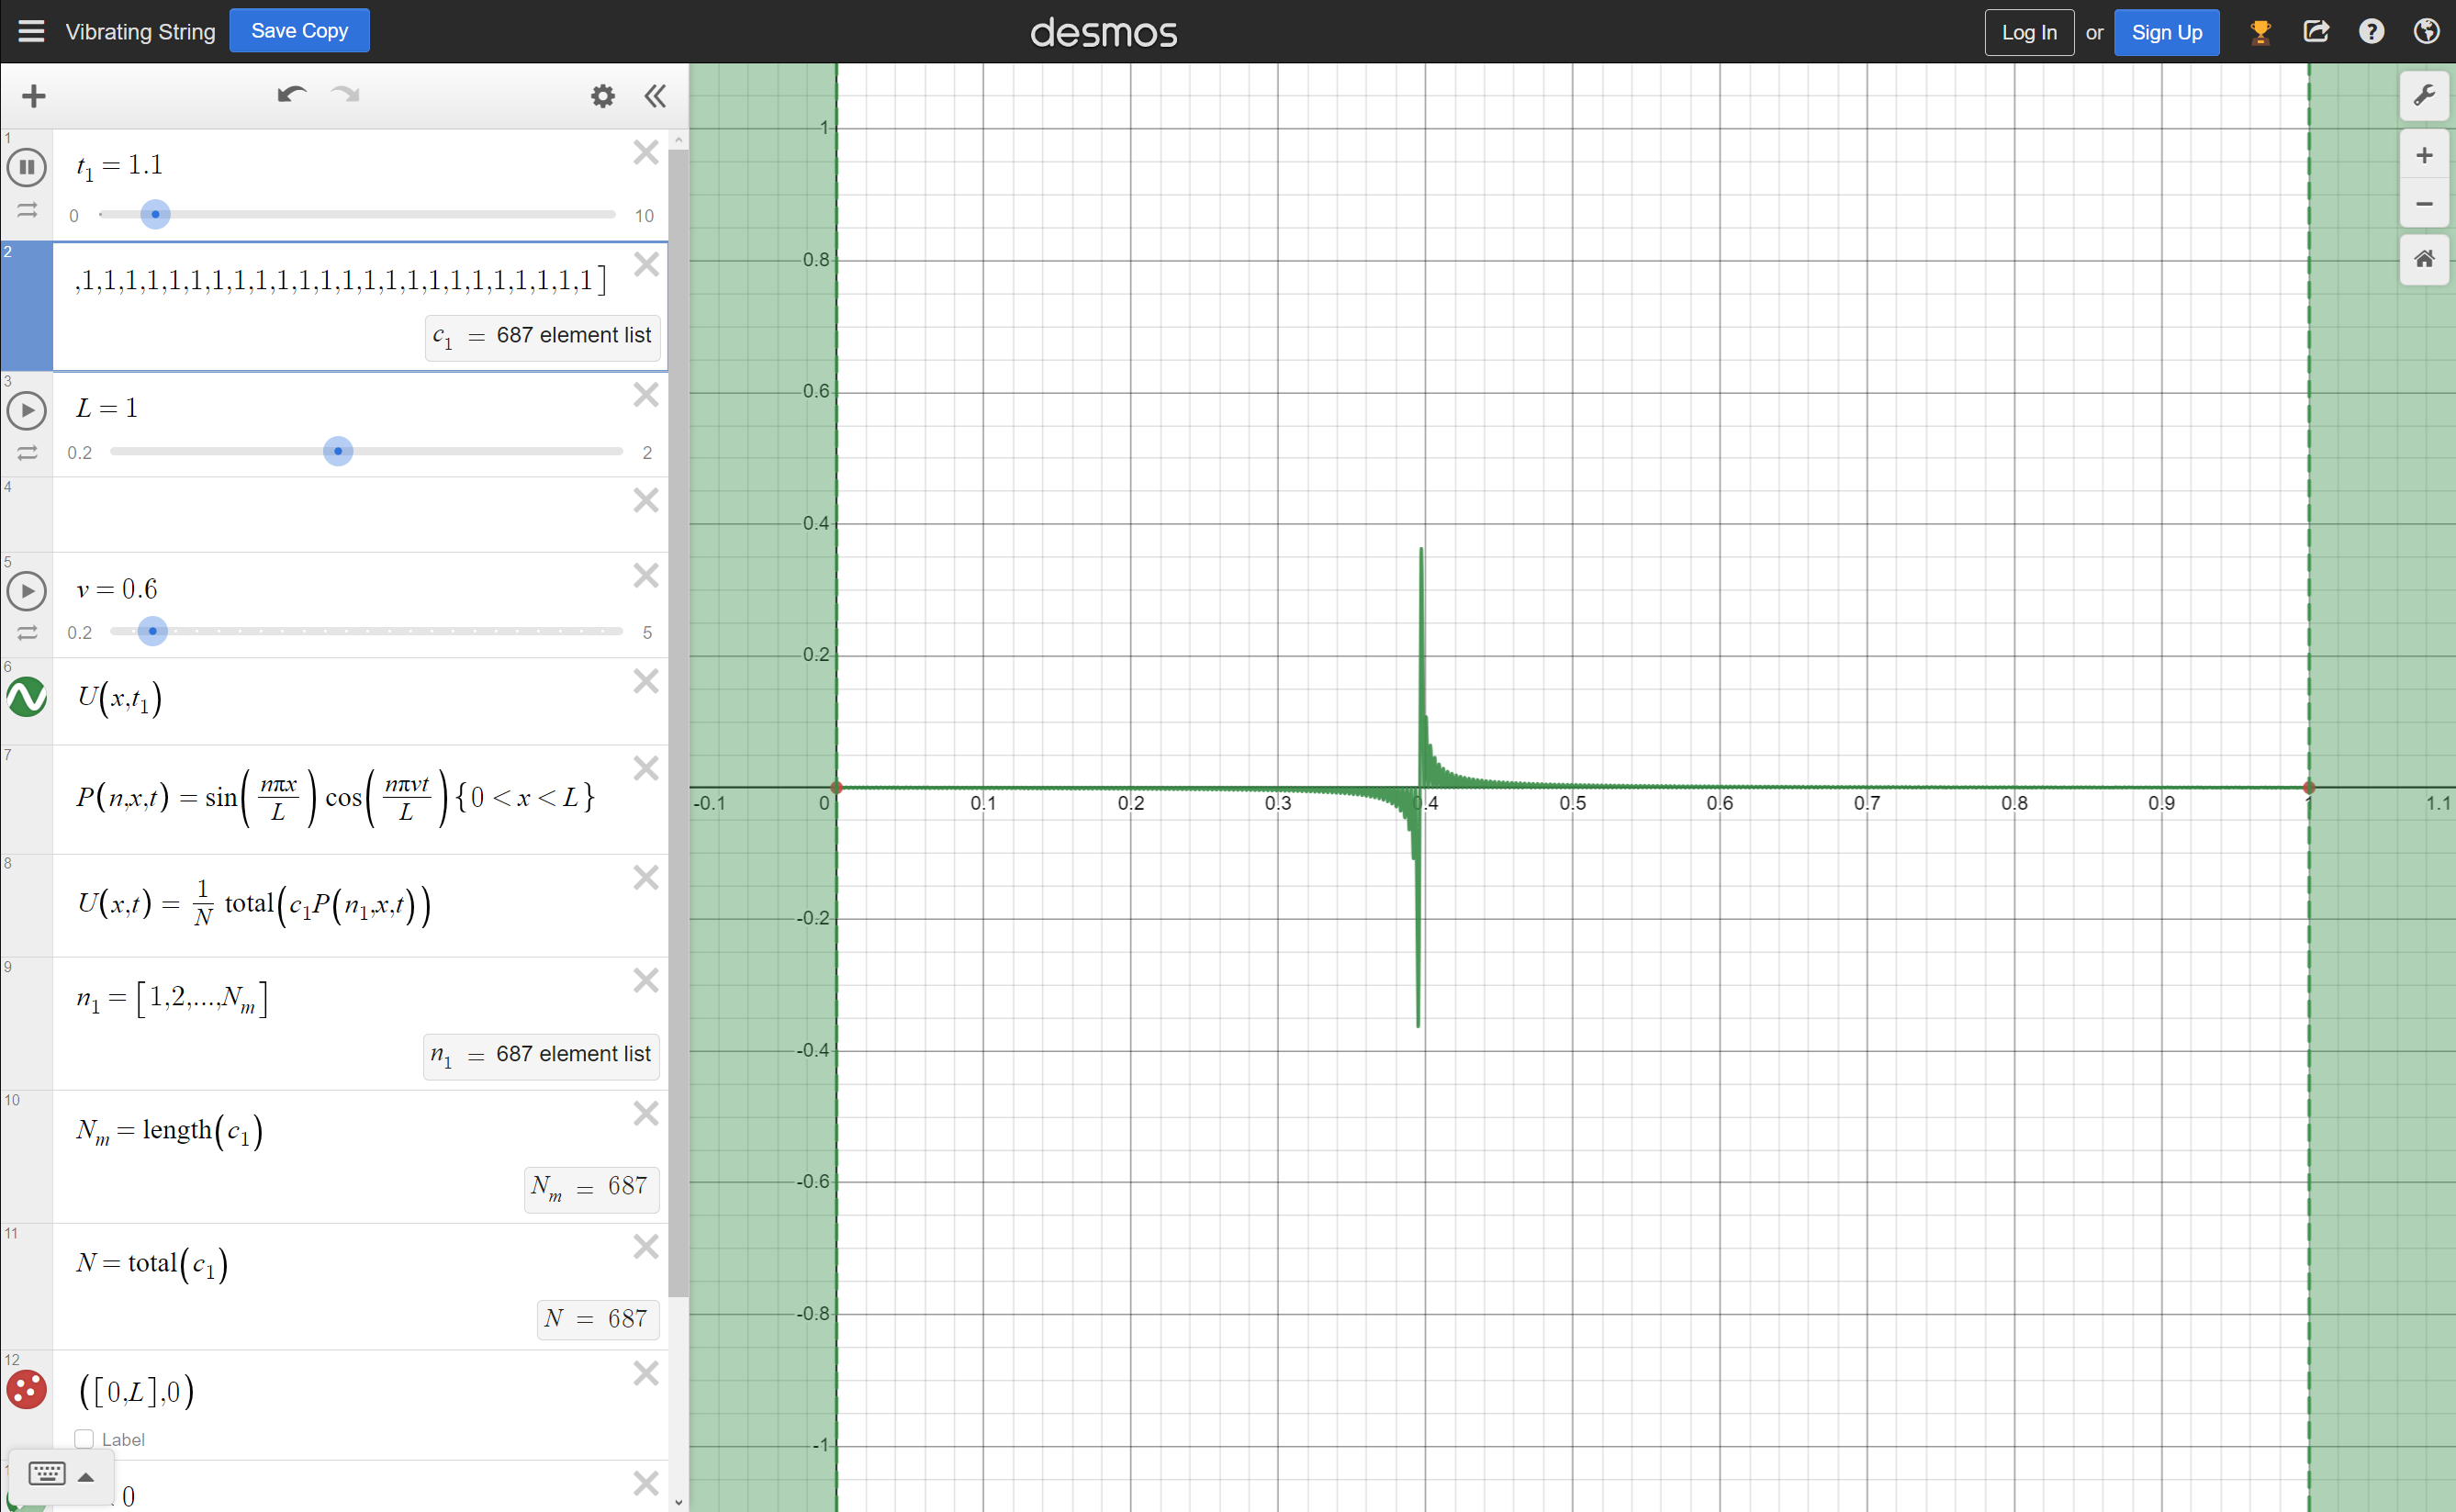
\includegraphics[scale=0.1]{Bilder/SamtaleTema1/Oppgave4b_2_prosjekt1.png}
    \caption{Figuren er hentet fra prosjekt i TFE4172, der mange bølger som løser TISE er lagt sammen for å produsere en kompakt bølgepakke. Produsert i desmos.}
    \label{fig:prosjekt1_eksempel}
\end{figure}

Som indikert til tidligere, henger HUP sammen med bølgepakker. Når bølger blir lagt sammen gir det utsving i en del av rommet, men selvom det fortsatt er en bølge er det en dårlig definert posisjon. 

Når vi måler bølgelengde/bevegelsesmengde vil vi kun få størrelsen fra en bølgene i bølgepakken, som da relativt til resten av bølgen er en viss usikkerhet ($\Delta p$). 

For mindre $\Delta x$ (mer nøyaktig posisjon) kreves flere bølger, men dette fører til støre $\Delta p$ (usikkert moment).

\subsection{Dobbelspalte eksperimentet}
\label{sec:tema1_9}
Isac Newton påstod at lys kun var bestående av partikler, men Thomas Young introduserte dobbelspalte ekperimentet. Eksperimentet gikk ut på å produsere en lyskilde, sende den gjennom to smale spalter som stod en avstand $d$ fra hverandre, og videre på en vegg bak (NB! viktig at disse avstandene er store relativ til spalteavstanden). For så å se om det dannet seg et mønster. I Youngs tilfelle så gjorde det det, og han var den første til å vise fenomenet inerferens. Det ga opphav til teorien om at lys hadde både partikkel egenskaper og bølge egenskaper.

Youngs eksperiment ble gjort i 1804, over hundre år før kvantemekanikken ble postulert, likevel er dobbelspalte eksperimentet essensielt til å vise at kvantepartikler innehar bølge egenskaper. Vi kan starte med å se på 3 eksempler, som bygger intuisjon for eksperimentet. Et med maskingevær kuler, vannbølger og sist lys.

\begin{figure}[!htb]
    \centering
    \includegraphics{Bilder/SamtaleTema1/maskingevær.png}
    \caption{Maskingevær som skytes mot to spalter.}
    \label{fig:Maskingevær}
\end{figure}

\begin{figure}[!htb]
    \centering
    \includegraphics{Bilder/SamtaleTema1/vannbølger.png}
    \caption{Plane Vannbølger som beveger seg mot to spalter.}
    \label{fig:vannbølger}
\end{figure}

\begin{figure}
    \centering
    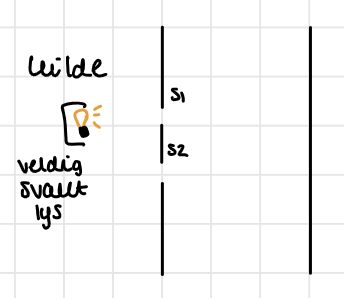
\includegraphics{Bilder/SamtaleTema1/lyskilde.png}
    \caption{Lyskilde som beveger seg mot to spalter, kan være en kontinuerlig lyskide eller eksitere atom slik at de sender ut fotoner (isåfall må man ha en film som tar imot denne energien, og det må være mørkt i rommet).}
    \label{fig:enter-label}
\end{figure}

\autoref{fig:resultaterDobbel} viser resultater fra dobbelspalte eksperimentet for de tre introduserte tilfellene. Vi ser at for maskingeværet vil det være tilfeldig spredning. for vannbølgen er resultatet som forventet, det oppstår destruktiv og konstruktiv interferens nå bølgen går gjennom. Så kommer vi til lyset, der et og et foton er ''skutt'' mot spaltene. Vi ser at det danner seg et interferens mønster, så lys har bølge egenskaper.

\begin{figure}[!htb]
    \centering
    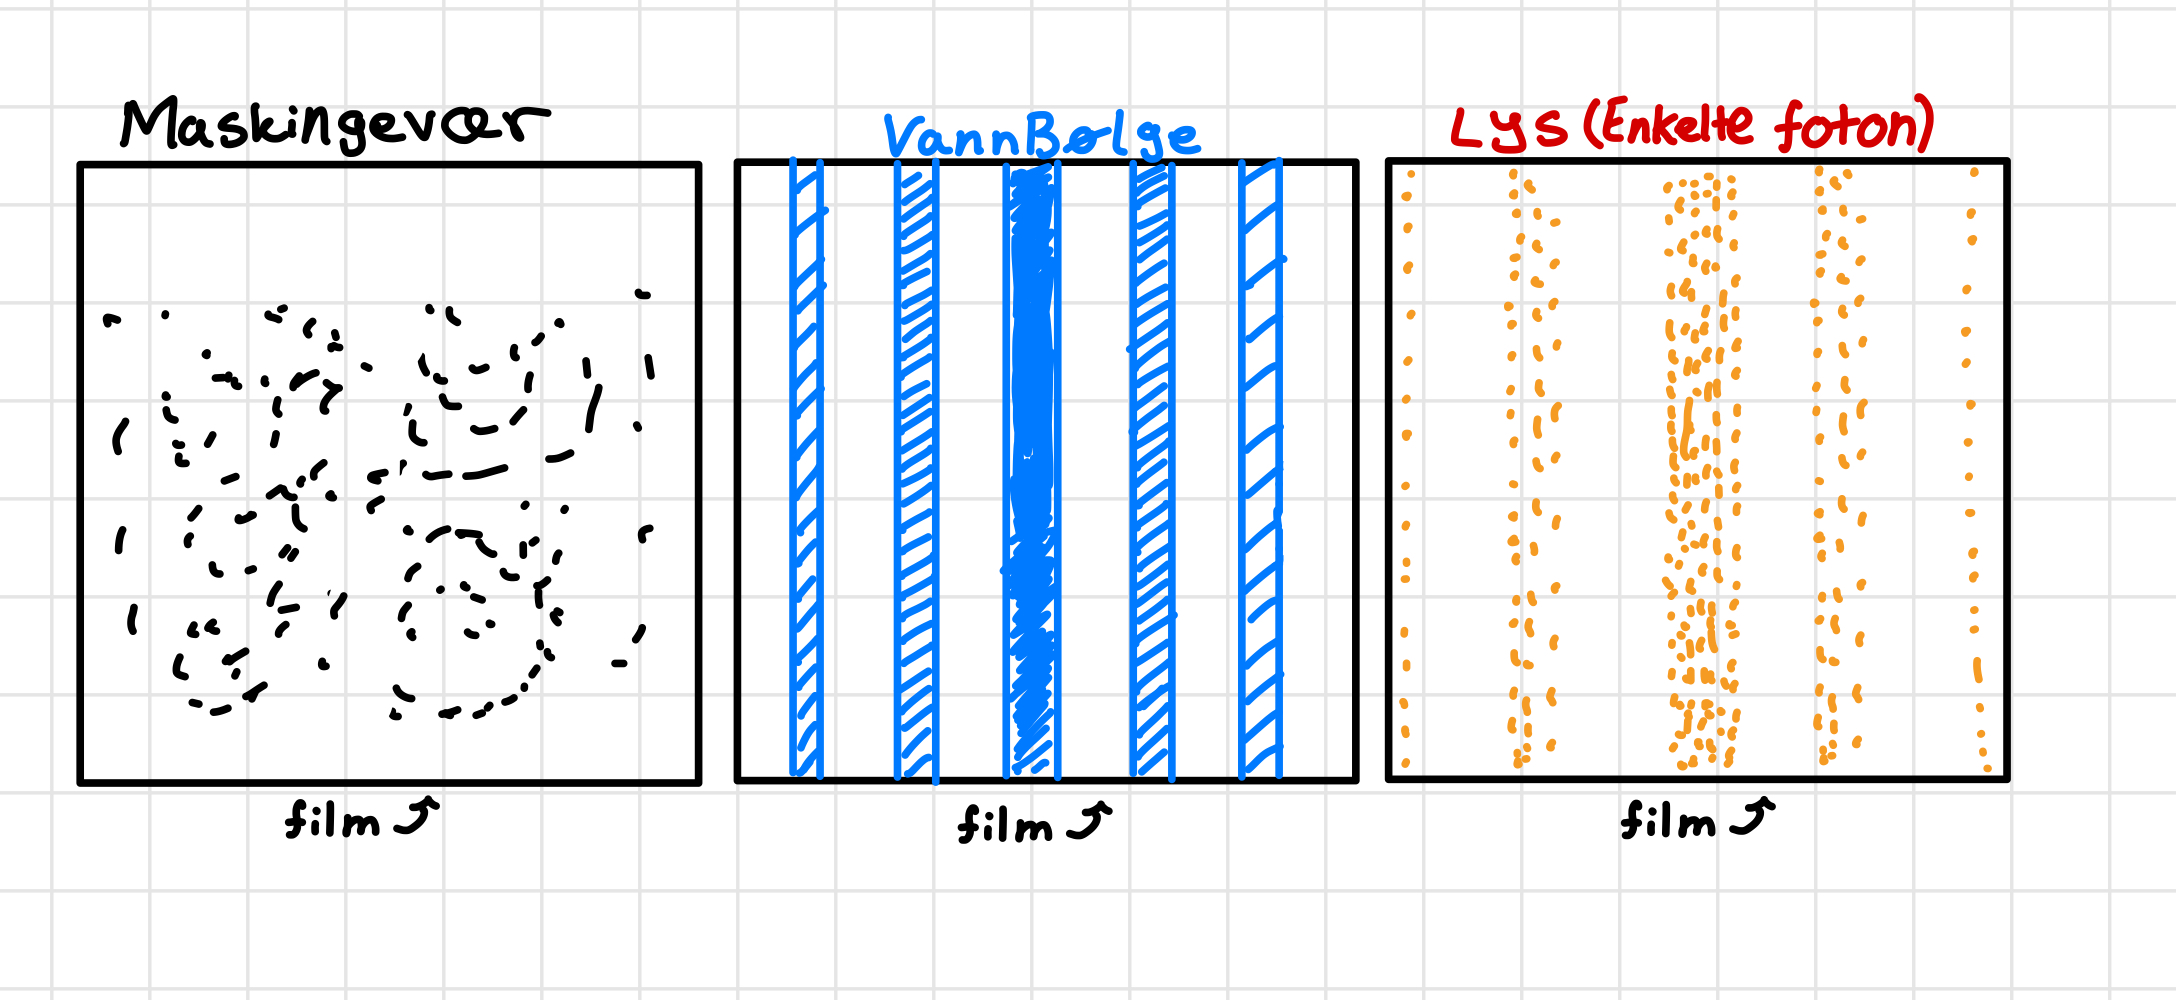
\includegraphics[scale=0.22]{Bilder/SamtaleTema1/ResultaterDobbelspalte.jpeg}
    \caption{Resultater fra dobbelspalte eksperimentet}
    \label{fig:resultaterDobbel}
\end{figure}

Vi kan si at interferens mønsteret som dannes er proporsjonal med $sinc$ funksjonen

\begin{equation}
    \label{eq:intensity}
    I(\theta) \thicksim I_0 (sinc(\beta))^2
\end{equation}

Nå er vel spørsmålet om kvantepartikler (elektron osv.) oppfører seg som bølger også? Det er litt komplisert, men vi prøver å forklare. La oss si at vi fører det samme eksperimentet vi hadde for lys. Når partikkelen skytes ut vil den inneha flere posisjoner samtidig i.e. den følger bølgefunksjonen og oppfører seg som en bølge, fra den treffer filmen og en ''måling'' blir tatt og vi avslører posisjonen som partikkelen har ''valgt''.

Nå kommer det som kanskje er litt vanskelig å skjønne, Hvis vi legger til en observator ved spaltene for å måle hvilken av de to spaltene partikkelen går gjennom, men da ser plutselig mønsteret på filmen mer ut som maskingevær fordelingen (!?) hvorfor det? Når vi tar en måling av partikkelen for å bestemme hvilken spalte den går gjennom, så må bølgefunksjonen kollapse, dette gjør at partikkeln må ''bestemme'' seg fr en posisjon og bevegelsesmengde. Det tar noen øyeblikk fra målingen er gjort til bølgefunksjonen gjenoppstår, og vi mister hele interferens mønsteret som egentlig skulle oppstått.

\begin{definition}
    \textbf{Bølge - partikkel dualiten: }om lys kan oppføre seg som partikler og bølger, kan partikler/materie oppføre seg som bølger.
\end{definition}